\section{Object Storage}
In Calico, all core components are stored using high performance Java hash maps. 
We decided that using FastUtil's \cite{fastutil} high performance maps would provide a better response time as opposed to using Java's core HashMap class. 
Each controller contains a single hash map that acts as a database for all objects that the controller is responsible for.
All access to hash maps requires use of a ``key'' to perform a lookup.
All objects are given a sequential 64-bit integer that acts as a globally unique identifier for each object.

One important design decision that was made was the choice to use a sequential identifier for each new object. The two factors that influenced our decision were: the relatively small size of a 64-bit integer in comparison with a universally unique string (which would be almost double the size), and better client performance.
Small size was very important to us as this identifier is included in nearly every network packet that is sent to and from the server. We wanted the footprint to be as small as possible, but we needed something that we could ensure would be unique for every object. 
The second decision -- better client performance -- was another benefit provided by using a sequential identifier. Clients can request a pre-allocated block of identifiers that they can assign to objects created client-side. The client can then create objects and assign them an identifier and submit the object directly to the server. Due to the fact that identifiers are pre-allocated, the client does not have to wait for confirmation from the server in order to add the object to its local hash map.


\begin{figure}[h!]
  \centering
  \begin{subfigure}[t]{0.4\textwidth}
    \centering
    \small
    \verbatiminput{figures/java/storage_stroke.java}
    \normalsize
    \caption{Stroke}
    \label{code:stroke_storage}
  \end{subfigure}%
  ~ 
  \begin{subfigure}[t]{0.4\textwidth}
    \centering
    \small
    \verbatiminput{figures/java/storage_scrap.java}
    \normalsize
    \caption{Scrap}
    \label{code:scrap_storage}
  \end{subfigure}
  \caption{Calico object representations}
  \label{code:storage}
\end{figure}

Figure \ref{code:storage} shows snippets from two objects within Calico. The first is the \texttt{Stroke} element (which provides lines) and the second is the \texttt{Scrap} object. A graphical depiction of scraps can be seen in Figure \ref{fig:scraps_storage} as the light gray areas. Scraps can be parented within other scraps (if a scrap is completely contained within another scrap, then the larger scrap would be considered the parent of the smaller scrap).

Figure \ref{code:storage} shows how all elements within Calico are provided with a unique 64-bit \texttt{uuid} which acts as the ID for the object. The second field, \texttt{parentUUID} is the ID value of the parent object that contains the current object. If the current object is not parented, then this would be set to \texttt{0L}. The third field is the \texttt{canvasUUID}. This value is always present, as it links the current element to the specific canvas that it was created on. Every element within Calico must be created on an existing canvas. 

The last field that is shared among Calico elements is the \texttt{points} field. We decided to use Java's native \texttt{Polygon} class to represent the coordinate path of the given element. By using a \texttt{Polygon} object, we are able to use native geometry operations to determine containment and intersection of elements. When a stroke is being drawn on a client machine, the server will continously append \texttt{Point2D} objects to the \texttt{points} field for the respective Stroke. 

The \texttt{Scrap} class shown in Figure \ref{code:scrap_storage} also includes three additional sets: \texttt{childScraps}, \texttt{childStrokes}, \texttt{childArrows}. These sets contain a list of UUIDs that can be mapped to any element that is a child of this scrap. These sets are accessed whenever a parent scrap is deleted or moved, because all operations must be executed on all child elements.


\begin{figure}[h!]
  \centering
  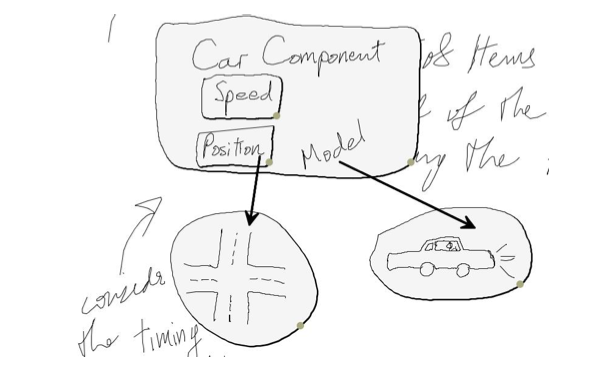
\includegraphics[width=0.8\textwidth]{scraps.png}
  \caption{Calico design session}
  \label{fig:scraps_storage}
\end{figure}

The screenshot shown in Figure \ref{fig:scraps_storage} displays a typical design session in Calico. This image represents a single \texttt{Canvas} object which would be stored within the \texttt{CanvasController} class. The \texttt{Canvas} object would have a list that contains the identifiers for each object that is being displayed on screen (five \texttt{Scrap}s, two \texttt{Arrow}s, and many \texttt{Stroke}s). Each of these objects is stored in their respective controller. Each of these objects requires a list of \texttt{Point}s that form the boundaries of the object. These are used within Calico to determine the location of an object, as well as whether an object is contained within another object (such as a scrap). Each object can have additional attributes that are specific to its type (arrows need endpoints, strokes have a color). These attributes are stored within the object itself and are converted to a \texttt{CalicoPacket} whenever a new client connects and needs to load the existing state of Calico.



